\documentclass[mathserif, aspectratio=169]{beamer}
%
%%%%%%%%%%%%%%%%%%%%%%%%%%%%%%%%%%%%%%%%%%%%%%%%%%%%%%%%%%%%%%%%%%%%%%%%
% need to split the includes to make spell checking work.
\usepackage{arev, arevmath}
\usepackage[scaled]{cabin}
\usepackage[T1]{fontenc}
\usepackage[super]{nth}
\usepackage{pifont}
\usepackage{wasysym}
\usepackage{tabularx}
\usepackage{array}
\usepackage{booktabs}
\usepackage{boldline}
\usepackage{colortbl}
%\usepackage{amsmath}
\usepackage{bm}
\usepackage{tcolorbox}
\usepackage{adjustbox}
\usepackage{minibox}
\usepackage{makecell}
\usepackage{adjustbox}
\usepackage{textcomp}
\usepackage[absolute,overlay]{textpos}
\setlength{\TPHorizModule}{1mm}%
\setlength{\TPVertModule}{1mm}%
\tcbuselibrary{skins}

\makeatletter
\newcommand{\antsize}{\@setfontsize{\antsize}{4pt}{4pt}}
\makeatother
\newcommand{\at}{\makeatletter @\makeatother}

\newcommand{\cmark}{\ding{51}}%
\newcommand{\bottomline}[1]{\vskip0pt plus 1fill{\alert{#1}\phantom{g}\vskip 1.0mm}}

\newcommand{\Quote}[2]{%
	\begin{center} 
		\begin{minipage}{0.7\textwidth} 
			\hrule
			\vskip 3mm
			\emph{{\color{ICTPblue} ``#1''}
			
			~~~~ {\color{ICTPorange} --- #2}}
			\vskip 3mm
			\hrule
			\vskip 2mm
		\end{minipage}
	\end{center}}


\mode<presentation>%
{
	\usetheme{default}
	%\usetheme[width=2.5cm]{PaloAlto}
	\usecolortheme{dove}
	\useoutertheme{infolines}
	% oder auch nicht

	% ICTP Colors
	\definecolor{ICTPblue}{RGB}{37,86,162} % 0x255682
	\definecolor{ICTPorange}{RGB}{255,130,0} % 0xff8200
	\definecolor{ICTPgreen}{RGB}{0,100,0}
	\definecolor{ICTPdark}{RGB}{80,80,80} % 0x505050
	\definecolor{ICTPlight}{RGB}{120,120,120}
	\definecolor{ICTPbrown}{RGB}{178,91,0}

	\definecolor{codebg}{rgb}{0.95,0.95,0.95}

	% Color theme
	\setbeamercolor{alerted text}{fg=ICTPorange}
	\setbeamercolor{frametitle}{fg=ICTPblue}
	\setbeamercolor{title}{fg=ICTPblue}
	\setbeamercolor{subtitle}{fg=ICTPorange}
	\setbeamercolor{normal text}{fg=ICTPdark}
	\setbeamercolor{author in foot}{fg=ICTPblue}
	\setbeamercolor{item}{fg=ICTPblue}
	\setbeamercolor{footline}{fg=ICTPblue}
	%\setbeamercolor{item projected}{bg=ICTPorange}
	%\setbeamercolor{item projected}{fg=white}

	\setbeamertemplate{headline}
	{}
	\setbeamertemplate{frametitle}
	{
		%\textbf{{\insertframetitle\phantom{g}}}\\
		%\textbf{\insertframetitle\phantom{g}}\\
		\textbf{\underline{\insertframetitle\phantom{g}}}\\
		%\textbf{\underline{\insertframetitle}}\\
		\vskip 1.0mm
		%{\color{UOLgold}\hrule height 2pt}
		%\par
	}
	\addtobeamertemplate{frametitle}{}{\vspace{-1em}}
	\setbeamertemplate{footline}{
		{%
			\textbf{ \hskip 3.0mm\insertshorttitle\phantom{.}---\phantom{.}\insertshortinstitute\hfill\insertframenumber\,/\,\inserttotalframenumber\hskip 3.0mm} 
		}
	}

	\setbeamertemplate{navigation symbols}{}%remove navigation symbols
	\setbeamertemplate{itemize items}[circle]
	\setbeamertemplate{enumerate items}[fg=ICTPblue]
	\setbeamercolor{itemize items}{fg=ICTPblue}
	\setbeamercolor{sidebar}{bg=ICTPblue}
	\setbeamercolor{title in sidebar}{fg=ICTPorange}
	\setbeamercolor{author in sidebar}{fg=ICTPorange}
	\setbeamercolor{section in sidebar}{fg=ICTPorange}
}

%\input{tikz/common-styles}

\usepackage{graphicx}
\usepackage[latin1]{inputenc}

\graphicspath{{../figs/}{../figs/common/}{../figs/islr/}}

\title[Statistical Learning] % (optional, nur bei langen Titeln n�tig)
{\textbf{Introduction to Statistical Learning\\ {\it with applications in Python}}\\%
		\href{www.statlearning.com}%
		{\tiny\it Based on ``Introduction to Statistical Learning, with applications in R'' by Gareth James, Daniela Witten, Trevor Hastie, Robert Tibishirani}\vspace{2em}}
		\vspace{-2.5cm}{}


		\author{\href{mailto:?to=Kurt Rinnert <kurt.rinnert@cern.ch>&subject=PWF Statistical Learning}{Kurt Rinnert}}

\institute[{\href{https://www.ictp.it/physics-without-frontiers.aspx}{Physics Without Frontiers} --- \href{https://www.ictp.it/}{ICTP}}] % (optional)
{\color{ICTPblue}\bfseries \href{https://www.ictp.it/physics-without-frontiers.aspx}{Physics Without Frontiers}\\\vspace{1mm}%
\href{https://www.ictp.it/}{
\includegraphics[width=0.20\textwidth]{common/ICTP-logo-full-trans.png}}\\%
\href{https://www.liverpool.ac.uk/physics/}{
\includegraphics[width=0.2\textwidth]{common/uol_logo.png}}}

\date{}

\titlegraphic{
	\texorpdfstring{\vspace{-2.8cm}}{}
	 \begin{minipage}[b][1.3cm][b]{0.26\textwidth}\color{ICTPlight}\antsize
		Copyright \textcopyright~2019\\
		\href{mailto:?to=Kurt Rinnert <kurt.rinnert@cern.ch>&subject=PWF Statistical Learning}{Kurt Rinnert <kurt.rinnert{\tt @}cern.ch>},
		\href{mailto:?to=Kate Shaw <kshaw@ictp.it>&subject=PWF Statistical Learning}{Kate Shaw <kshaw{\tt @}ictp.it>}\\
		Copying and distribution of this file, with or without modification,
		are permitted in any medium without royalty provided the copyright
		notice and this notice are preserved.  This file is offered as-is,
		without any warranty.


		Some of the figures in this presentation are taken from ``An Introduction to
		Statistical Learning, with applications in R''  (Springer, 2013) with
		permission from the authors: G. James, D. Witten,  T. Hastie and R. Tibshirani 
	 \end{minipage}\hspace{10cm}
}


\addtocounter{framenumber}{-1}

% nicer table row separation
\renewcommand{\arraystretch}{1.2}

% color boxes
\newcommand{\tabboxset}{\tcbset{enhanced, nobeforeafter, boxrule=0pt, boxsep=0pt, colback=codebg, colframe=codebg, coltext=ICTPdark, rounded corners, arc=4pt, fonttitle={\bfseries\tiny}}}
\newcommand{\codeboxset}{\tcbset{enhanced, nobeforeafter, boxrule=0pt, boxsep=0pt, colback=codebg, colframe=codebg, coltext=ICTPdark, rounded corners, arc=4pt, fonttitle={\bfseries\tiny}}}

\newcommand{\orange}{\color{ICTPorange}}
\newcommand{\blue}{\color{ICTPblue}}
\newcommand{\dark}{\color{ICTPdark}}
\newcommand{\R}{\mathbb{R}}
\newcommand{\dat}[1]{{\footnotesize\tt\orange #1}}
\newcommand{\e}[1]{\emph{#1}}
\newcommand{\bh}{\hat{\beta}}
\newcommand{\h}{\hat}

\makeatletter
\newcommand{\includegraphicsdpi}[3]{%
	\pdfimageresolution=#1%
	\includegraphics[#2]{#3}%
	\pdfimageresolution=72%
}

\newenvironment{blurb}%
	{\begin{center}\begin{minipage}{0.6\textwidth}\footnotesize}
	{\end{minipage}\end{center}}

\newenvironment{cpage}%
	{\begin{center}\begin{minipage}{0.75\textwidth}}
	{\end{minipage}\end{center}}

\newenvironment{popblock}[2]%
	{\begin{center}\begin{minipage}{#1}\footnotesize
		\begin{tcolorbox}[colframe=codebg, colback=white, colupper=ICTPdark, title={\normalsize\bfseries\blue #2}]}
	{\end{tcolorbox}\end{minipage}\end{center}}
\makeatother

\subtitle{\bfseries%
  {Linear Regression}\\%
  {\tiny\it linear models, least square fit, simple \& multiple linear regression, qualitative predictors}\\%
}
\begin{document}
\frame[plain]{
	\vskip 1.0mm
	\titlepage
	\vskip 1.0mm
}


\begin{frame}{Abstract}

	\begin{blurb}
		Linear models are an important topic in statistical learning.  

		The true relationships between predictors and responses are rarely linear.
		But linear models often provide reasonable approximation. They provide
		high interpretability and have low variance, mitigating the risk of over-fitting.
		Linear models can be extended to include (some) non-linear relationships. 

		Linear models also provide an excellent baseline to compare other models against: if 
		our sophisticated model does not do much better than a linear model we might consider
		trading some bias for lower variance.
	\end{blurb}
\end{frame}

\begin{frame}{Overview}
	\begin{itemize}
		\item Simple linear regression.
		\item Multiple linear regression.
		\item Qualitative predictors.
		\item Extensions to the linear model.
	\end{itemize}
	\bottomline{This will require some mathematics.}
\end{frame}

\begin{frame}{The Advertising Data Set}
	\begin{center}
		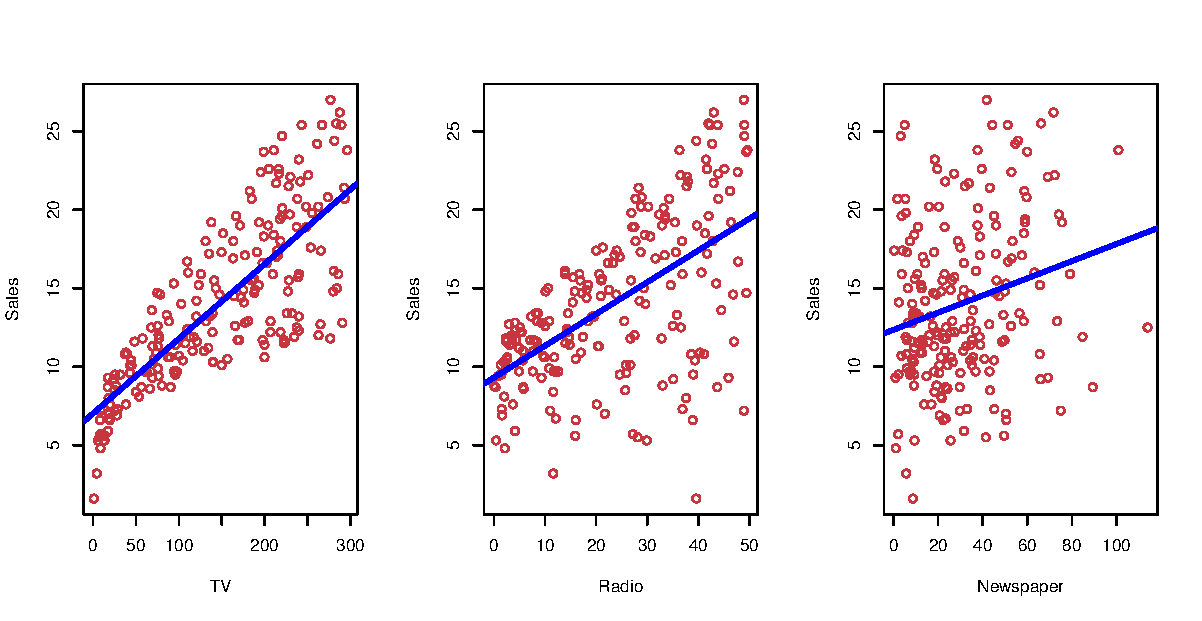
\includegraphics[width=0.6\textwidth]{2_1}

		We want to understand how \dat{sales} depends on \dat{TV}, \dat{radio} and \dat{newspaper}.
	\end{center}
	\bottomline{We will use this data set to illustrate the concepts in this lecture.}
\end{frame}

\begin{frame}{Interesting Questions}
	\begin{enumerate}
		\item Is there a relationship between advertising budget and sales?
		\item How strong is the relationship between advertising budget and sales?
		\item Which media contribute to sales?
		\item How accurately can we estimate the effect of each medium on sales?
		\item How accurately can we predict future sales?
		\item Is the relationship linear?
		\item Is there synergy among the advertising media?
	\end{enumerate}
	\bottomline{Linear regression can answer all of these questions.}
\end{frame}

\begin{frame}{Simple Linear Regression}
	\begin{itemize}
		\item Simple linear regression assumes an approximate simple linear relationship between\\
			one predictor and the response:
			\[ Y \approx \beta_0 + \beta_1 X \]
		\item For example, $X$ might represent the \dat{TV} budget and $Y$ might represent \dat{sales}:
			\[ \text{\dat{sales}} \approx \beta_0 + \beta_1\times\text{\dat{TV}} \]
		\item The \e{coefficients}, or \e{parameters}, $\beta_0$ and $\beta_1$ are the \e{intercept} and
			\e{slope} of a line.
		\item We can \e{estimate} the parameters from the training data and \e{predict} \dat{sales}\\
			from the \dat{TV} budget.
			\[ \hat{y} = \hat{\beta}_0 + \hat{\beta}_1 x \]
	\end{itemize}
	\bottomline{We use the \e{hat} symbol, $\;\bm{\hat{}}\;$, to denote estimates and predictions.}
\end{frame}

\begin{frame}{Estimating the Coefficients}
	\begin{itemize}
		\item In practice, $\beta_0$ and $\beta_1$ are unknown.
		\item Given the training data 
			\[ (x_1, y_1), (x_2, y_2), \dots, (x_n, y_n) \]
			we want to obtain estimates of the coefficients $\beta_0$ and $\beta_1$ such that
			\[ y_i \approx \hat{\beta}_0 + \hat{\beta}_1 x_i,\;\; \forall i = 1,\dots,n \]
		\item In other words we want to find $\hat{\beta}_0$ and $\hat{\beta}_1$ such that the
			resulting line is as close\\
			as possible to the $n = 200$ observations in the \dat{Advertising} data set.
	\end{itemize}
	\bottomline{We need to define what we mean by ``close''.}	
\end{frame}

\begin{frame}{Residual Sum of Squares}
	\begin{itemize}
		\item Given the predictions of $Y$ for the $i$th value of $X$
			\[ \hat{y}_i = \hat{\beta}_0 + \hat{\beta}_1 x_i \]
			we define the $i$ith \e{residual} as
			\[ e_i = y_i - \hat{y}_i \]
		\item The \e{residual sum of squares} is then
			\[ \text{RSS} = e_1^2 + e_2^2 + \dots + e_n^2 \]  
			or equivalently
			\[ \text{RSS} 
				= (y_1 - \hat{\beta}_0 - \hat{\beta}_1 x_1)^2 
				+ (y_2 - \hat{\beta}_0 - \hat{\beta}_1 x_2)^2
				+ \dots
				+ (y_n - \hat{\beta}_0 - \hat{\beta}_1 x_n)^2\] 
	\end{itemize}
	\bottomline{A least squares fit minimises the RSS.}
\end{frame}

\begin{frame}{Least Squares Fit}
	\begin{itemize}
		\item The \e{least squares} approach chooses $\hat{\beta}_0$ and $\hat{\beta}_1$
			to minimise the RSS.
		\item Using some calculus and sum manipulation we can show that the optimal\\
			parameter estimates are:
				\begin{align*}
					\hat{\beta}_1 &= \frac{\sum_{i=1}^n (x_i - \overline{x})(y_i - \overline{y})}
					{\sum_{i=1}^n (x_i - \overline{x})^2}\\
					\phantom{a} & \phantom{b} \\
					\hat{\beta}_0 &= \overline{y} - \hat{\beta}_1 \overline{x}\\
				\end{align*}
	\end{itemize}
	\bottomline{Buckle up, we are going to prove it.}
\end{frame}

\begin{frame}{Least Squares Fit}
	\begin{center}
		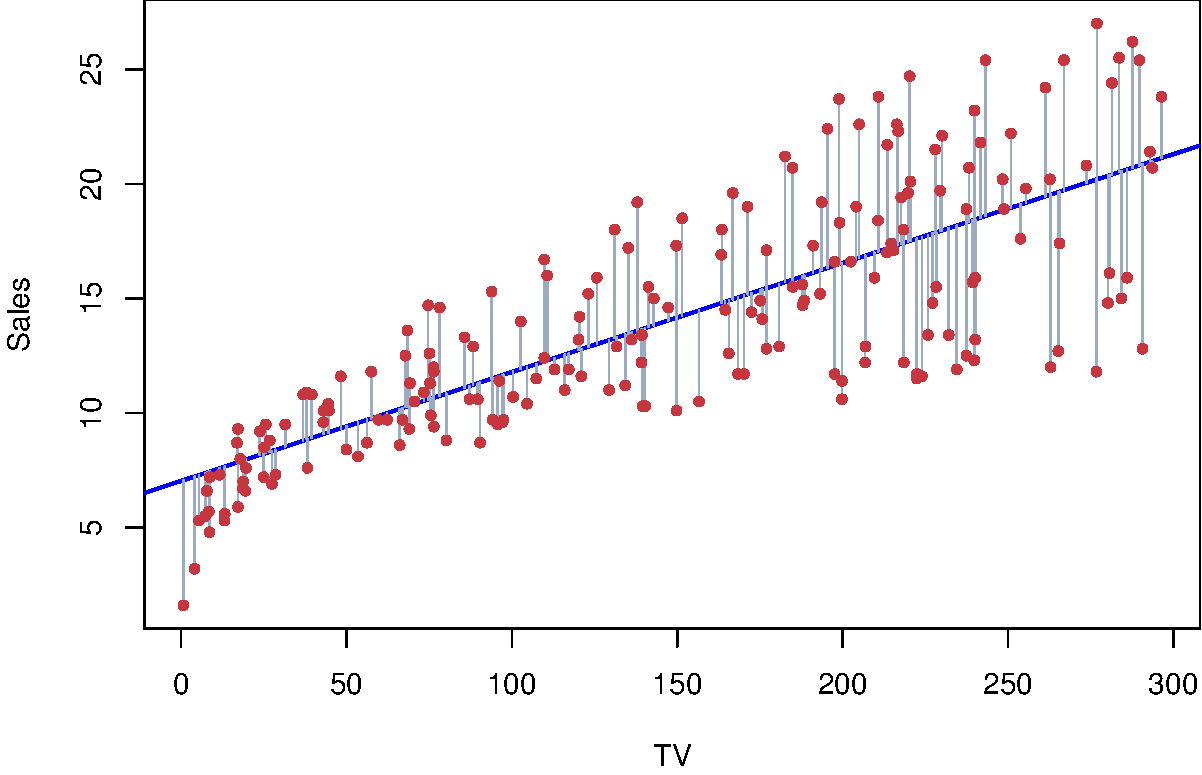
\includegraphics[width=0.6\textwidth]{3_1}

		Result of the least squares fit for the regression of \dat{sales} onto \dat{TV}.
	\end{center}
\end{frame}

\begin{frame}{Least Squares Fit}
	\begin{center}
		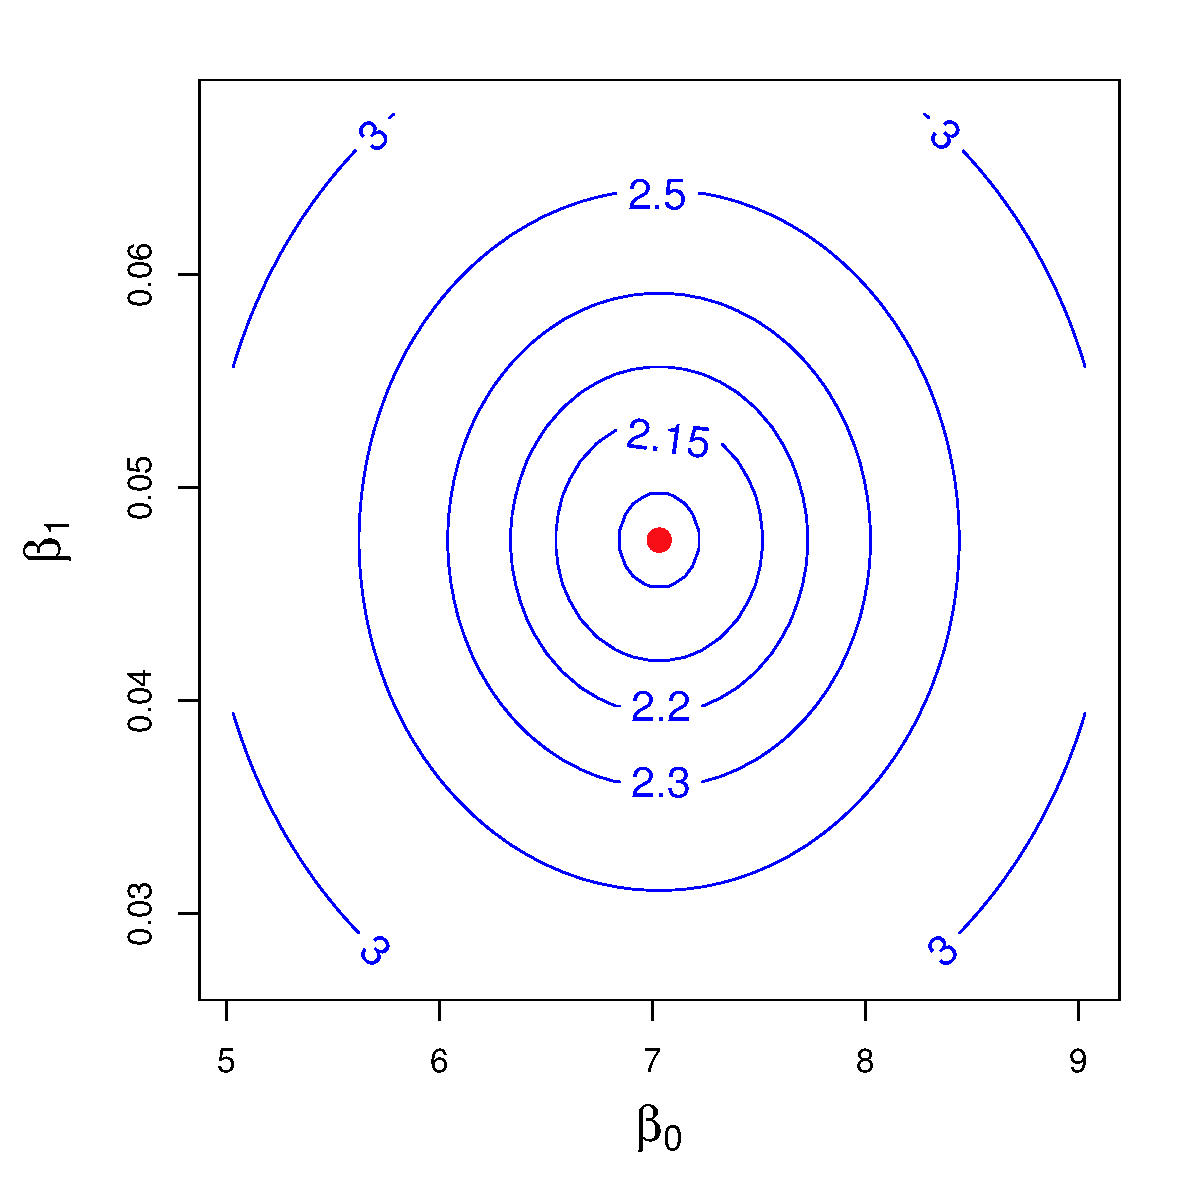
\includegraphics[width=0.4\textwidth]{3_2a}
		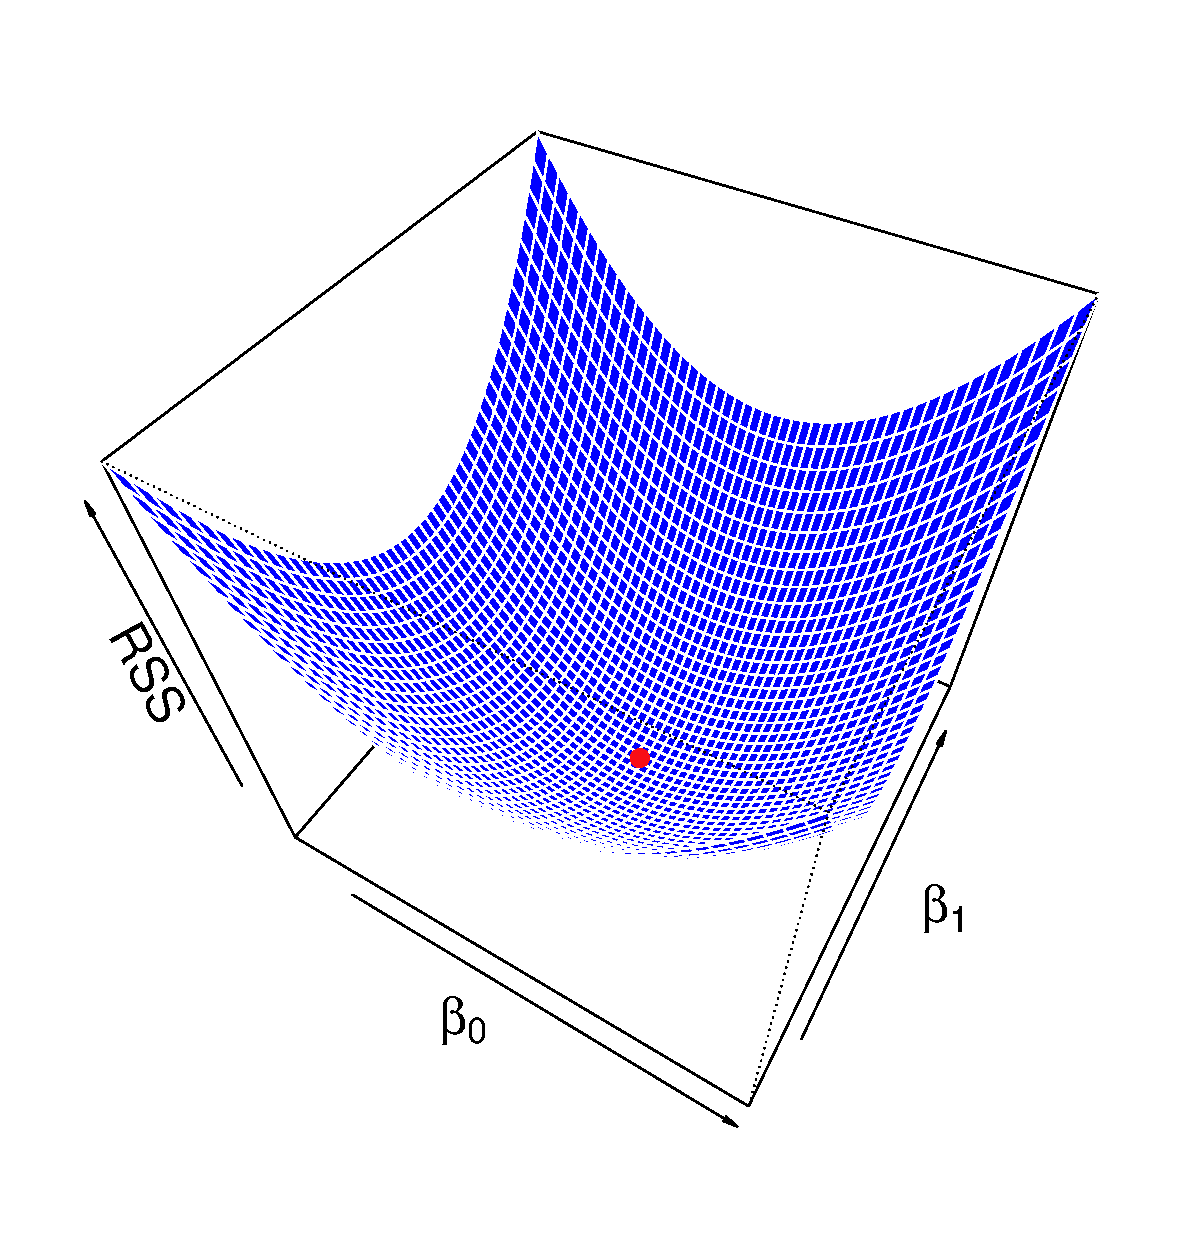
\includegraphics[width=0.4\textwidth]{3_2b}

		The RSS with \dat{sales} as the response and \dat{TV} as the predictor. The red dot marks the optimum.
	\end{center}
\end{frame}

\begin{frame}{Assessing Accuracies}
	\begin{itemize}
		\item We want to \e{quantitatively} answer two rather important questions: 
	\end{itemize}
	\begin{cpage}
		\begin{enumerate}
			\item \e{\orange Is there a relationship between the predictor and the response?}
			\item \e{\orange To what extend does our model fit the data?}
		\end{enumerate}
	\end{cpage}
	\begin{itemize}
		\item To this end, we need to clarify a few concepts. In particular the notions of \e{population},
			\e{sample} and \e{degrees of freedom}.
		\item Then we introduce a number of so-called \e{statistics}. Simply put, these are useful quantities
			we can compute from our data.
		\item It is beyond the scope of this course to formally justify all of this, but we will now
			spend some time to develop some intuition.
	\end{itemize}
	\bottomline{For this interlude we will look at the simpler problem of estimating a mean.}
\end{frame}

\begin{frame}{Populations}
	\begin{itemize}
		\item We (somewhat sloppily) define a \e{population} as the \e{full set} of potential observations.
		\item That could be an actual population (as in everyday language) like, say, the population\\
			of \e{all} \href{https://en.wikipedia.org/wiki/Blue\_whale}{\blue\underline{blue whales}} 
			alive on Earth today.
		\item It can also be the full set of instances of any abstract entity.
		\item We then might be interested in measuring a certain property of the instances in the population.
		\item For example, the \dat{length} of all blue whales alive on Earth today.
		\item Often we want to summarise our findings rather than presenting a raw data table \\
			(or graphical representation thereof). 
		\item A common way to summarise the data is reporting the \e{mean} and the \e{variance} of the 
			quantity of interest.
	\end{itemize}
	\bottomline{Note that there is nothing wrong with reporting the full distribution!}
\end{frame}

\begin{frame}{Samples}
	\begin{itemize}
		\item In practice, it is generally not possible to access the whole population.
		\item Quite literally, we don't have access to \e{all} blue whales.
		\item But we can look at a \e{sample} of the full population.
		\item The sample is a subset of the population we have access to.
		\item We generally assume the sample to be a \e{random sample}.
		\item Then we can try to \e{estimate} the mean and variance of the quantity of interest\\
			from the sample.
		\item Clearly, our estimates will \e{not} yield the \e{true} values of the mean and the variance.
	\end{itemize}
	\bottomline{Our goal is to avoid any \e{bias} in the estimates and evaluate their \e{accuracy}.}
\end{frame}

\begin{frame}{Estimating the Mean}
	\begin{itemize}
		\item If we had access to the whole population we could calculate the \e{true} mean $\mu$.
		\item Sadly, we have only access to a sample of $n$ observations.
		\item So all we can do is produce an estimate $\hat{\mu}$.
			\[ \hat{\mu} = \sum_{i=1}^n x_i \]
		\item This is the best possible estimate we can draw from a random sample.
		\item Intuitively, this is obvious from the fact that $\hat{\mu} = \mu$ if the sample covers
			the entire population.
	\end{itemize}
	\bottomline{It is \e{very} important that the sample is random. Beware of \e{selection bias}!}
\end{frame}
\end{document}
